\documentclass{beamer}
\ifxetex
 \usepackage{fontspec}
\else
 \usepackage[T1]{fontenc}
 \usepackage[utf8]{inputenc}
 \usepackage{lmodern}
\fi
\usepackage{amsmath, pdfpages, pdflscape, lscape, color, listings, hyperref, amssymb,graphicx,textcomp,varioref,afterpage,subcaption, float,color} 


% \makeatletter
% \def\input@path{{/home/simen/Dropbox/phd/presentations/presentations/neuronify}}
% %or: \def\input@path{{/path/to/folder}{/path/to/other/folder}}
% \makeatother

\title{Neuronify: a new tool for creating simple neural networks}
\author{Simen Tennøe,\newline Svenn-Arne Dragly,\newline Andreas V. Solbr\aa,\newline Milad H. Mobarhan}

\usetheme{cinpla3}


\begin{document}
\maketitle

\begin{frame}
  \frametitle{In this lecture we will introduce Neuronify, a new tool for creating neural networks}

  \begin{tikzpicture}[remember picture,overlay]  
    \node [xshift=-3.5cm,yshift=1.5cm] at (current page.center)
          {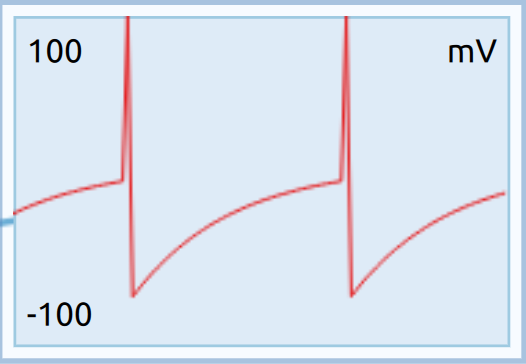
\includegraphics[width = 0.14\paperwidth ]{integrate.png}};
    \node [xshift=-2.cm,yshift=1.5cm, right] at (current page.center)
          { Integrate and fire neurons};
  \end{tikzpicture}

  \begin{tikzpicture}[remember picture,overlay]  
    \node [xshift=-2cm,yshift=-.5cm] at (current page.center)
          {
\includegraphics[width = 0.12\paperwidth ]{logo.png}};
    \node [xshift=1cm,yshift=-.5cm, left] at (current page.center)
          { Neuronify };
  \end{tikzpicture}

  \begin{tikzpicture}[remember picture,overlay]  
    \node [xshift=-.5cm,yshift=-2.5cm] at (current page.center)
          {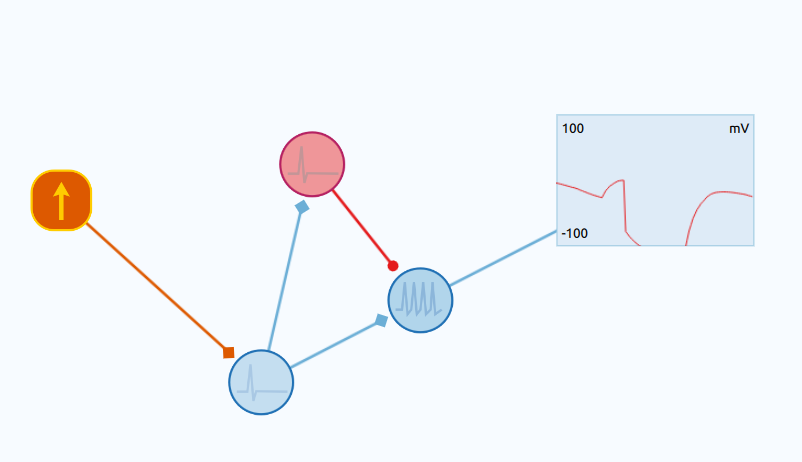
\includegraphics[width = 0.2\paperwidth ]{exercises.png}};
    \node [xshift=2.8cm,yshift=-2.5cm, left] at (current page.center)
          { Exercises};
  \end{tikzpicture}

\end{frame}



\begin{frame}
\frametitle{The general idea behind the integrate and fire model is a simple RC circuit that is shortcircuted once a threshold is reached}

\begin{figure}
\includegraphics<1>[width = 0.5\textwidth]{rcA.png}
\includegraphics<2>[width = 0.5\textwidth]{rcAI.png}
\includegraphics<3>[width = 0.5\textwidth]{rcARm.png}
\includegraphics<4>[width = 0.5\textwidth]{rcAEm.png}
\includegraphics<5>[width = 0.5\textwidth]{rcACm.png}
\includegraphics<6>[width = 0.5\textwidth]{rcAs.png}
\includegraphics<7>[width = 0.5\textwidth]{rcB.png}
\includegraphics<8>[width = 0.5\textwidth]{rcBs.png}
\end{figure}

\end{frame}



\begin{frame}
\frametitle{The integrate and fire neuron model is one of the simplest neuron models that exist and are therefore good  for modeling network}

\begin{itemize}[<+->]
\item Each neuron is fast to evaluate
\item For a network the precision of a single neuron is not important
\end{itemize}

\end{frame}

\begin{frame}
\frametitle{Neuronify is a new tool for creating neural networks}
\end{frame}

\begin{frame}
\frametitle{Exercises: create a network that gives a signal when a lightsource is moving right to left, but not the left to right}

\begin{block}{Exercise 1}
Start with a linear array of light-sensitive neurons that can be connected with each other through lateral inhibition, and which converge onto one output neuron, create a network that allows the output neuron to selectively respond to a spot of light that moves from left to right but not a spot of light that moves from right to left. 
\end{block}

\onslide <2> {\begin{block}{Clue} Use lateral inhibitory connections in one direction only.\end{block}}
\end{frame}

\begin{frame}
\frametitle{Exercises: create a network that }

\end{frame}


\end{document}
